\documentclass[a4paper]{article}

\usepackage{fullpage}
\usepackage{amsmath}
\usepackage{amsthm}
\usepackage{amssymb}
\usepackage{listings}
\usepackage{parcolumns}
\usepackage{graphicx}
\usepackage{todonotes}

\title{An instantiation algorithm for TLA+ expressions}
\author{}

\makeatletter
\let\ltxxlabel\ltx@label
\makeatother

\newcommand{\assignment}[1]{\{#1\}}
\newcommand{\inst}[2]{#1 {\leftarrow} #2}
\newcommand{\einst}[3]{#1 \stackrel{#2}{\Leftarrow} #3}
\newcommand{\tlaplus}[0]{{TLA+}}
\newcommand{\tla}[1]{#1}

\newcommand{\dor}{\textbf{or}}
\newcommand{\fpsubstin}[1]{\{#1\}}
\newcommand{\fpscat}[0]{\circ}
\newcommand{\substin}[2]{[#1:#2]}
\newcommand{\fpwith}{\leftarrow}
\newcommand{\fpwithout}[0]{\backslash}
\newcommand{\fpwithoutset}[1]{\backslash\{#1\}}
\newcommand{\iwith}{\leftarrow}
\newcommand{\metavar}[1]{\mathbf{#1}}
\newcommand{\rewrites}[0]{\;\rightarrow\;}

\newtheorem{lemma}{Lemma}

\newcommand{\sidebyside}[2]{
  \begin{minipage}{0.45\linewidth}
    #1
  \end{minipage}
  \hspace{10pt}
  \begin{minipage}{0.45\linewidth}
    #2
  \end{minipage}
}

\lstdefinelanguage{tlaplus}{
  morekeywords= { MODULE, LET, IN, VARIABLE, VARIABLES, CONSTANT, CONSTANTS,
    ASSUME, NEW, PROVE, THEOREM, LEMMA, ENABLED, ==, INSTANCE, BY, DEF },
  sensitive=true,
  morecomment=[l]{\*},
  morecomment=[s]{(*}{*)},
  morestring=[b]",
  literate={~} {$\sim$}{1},
  columns=fullflexible,
  basicstyle=\small
}

\lstset{language=tlaplus}

\begin{document}

\maketitle

\section{Overview}
\label{sec:overview}
\tlaplus{} has two kinds of substitution: instantiation of modules, which
preserves validity, and beta-reduction of lambda-expressions, which does not
necessarily preserve validity. Following the notions of SANY, we distinguish
three kinds of variables: temporal constants and temporal variables are
bound by instantiation whereas formal parameters are bound by lambda
abstraction. Furthermore, ENABLED binds all temporal variables within its
argument which are in the context of the next state operator '.

In the presence of unresolved instantiations or substitutions, it is often
unclear, which operator binds the occurrence of a particular temporal variable:
when we consider the expression
\tla{$(\lambda\; fp : ENABLED\; (fp \# fp'))(x)$}, it seems that the variable
$x$ is bound in the module. But in the beta-reduced form $ENABLED\; (x \# x')$
of this expression, only the first occurrence of $x$ is bound by the
module but its second (primed) occurrence is bound by ENABLED\footnote{To
  prevent complications from renaming, we will not assume alpha equivalence but
  will handle the renaming of bound variables explicitly.}.

Furthermore, the two substitutions do not commute. For example, let us
consider modules Foo and Bar:

\begin{parcolumns}{2}
  \colchunk{
    \begin{lstlisting}
      ---- MODULE Foo ----

      VARIABLE x

      E(u) == x' # u'
      D(u) == ENABLED ( E(u) )

      THEOREM T1 == D(x)

      ====
    \end{lstlisting}
  }
  \colchunk{
    \begin{lstlisting}
      ---- MODULE Bar ----

      VARIABLE y

      I == INSTANCE Foo with x <- y


      THEOREM T2 == I!D(y)

      ====
    \end{lstlisting}
  }
\end{parcolumns}

\vspace{2mm}
\noindent
It looks like \tla{I!T1} and \tla{T2} talk about the same formula \tla{D(y)},
but this is not the case: the first can be read as \tla{I!(D(y))}\footnote{This
  is not valid \tlaplus{} syntax.} and the second as \tla{(I!D)(y)}. In other
words, it makes a difference if we beta-reduce first or if we instantiate
first. Reducing D(x) first leads to \tla{ENABLED (x' \# x')}, which --
following the renaming instuctions in ``Specifying Systems'' -- becomes
\tla{ENABLED (\$x' \# \$x')} by the instantiation of \tla{x} with \tla{y},
because primed occurrences of \tla{\$x} are bound by their enclosing ENABLED,
not by the instantiation.

Instantiating first keeps the occurrence of the  formal parameter \tla{u} intact,
leading to \tla{I!D(u) == ENABLED ( u \# \$x') } but reducing the application
\tla{I!D(y)} leads to \tla{ENABLED (y' \# \$x')}. Now it is clear that
\tla{I!(D(y))} is unsatisfiable while \tla{(I!D)(y)} is valid.\footnote{ Since
  one of the axioms  of \tlaplus{} is that (TRUE \# FALSE), we can always find
  a domain element different from $x$. In fact, the axioms of set-theory even
  enforce denumerable models.}.

In the following, we will develop algorithms for both kinds of substitutions.
Since the occurrence of a lambda reducible expression (redex) as a subterm of
an instantiation may block the evaluation of the latter, inner substitutions
(i.e. those closer to the leaves of the term tree) must be evaluated before
outer ones. Definitions will also need special consideration because
we allow some of them to stay folded. But since a definition can contain
substitutions, they can not be treated like temporal constants.\footnote{
  Actually, already a definition \tla{D(x) == e} contains a substitution
  because it is equivalent to D == LAMBDA x : e.
}

\section{New Attempt: Explicit substitutions}

The original idea here is to represent both beta-reduction and instantiation
explicitly in the term graph. Then the two formulas in the introduction
could be written as D(u)\{u $\mapsto$ x\}[x $\mapsto$ y] and
D(u)[x $\mapsto$ y]\{u $\mapsto$ y\}, where reduction is denoted by curly
braces and instantiation is denoted by square braces. Actually, the SANY
data-structures allow to write reduction as application to an abstraction:
D(u)\{u $\mapsto$ x\} is then just \tla{(LAMBDA u: D(u))(x)}. Again, this
is not legal \tlaplus{} but allowed by SANY. Nevertheless, having an explicit
substitution nodes drastically simplifies the formal treatment of the
behavior\footnote{For instance, we rely on the fact that the permutation
  of explicit substitutions to the leaves of the term tree preserves their
  idempotence. The explicit substitution nodes are also vital to the
  termination proof of the permutation algorithm.
}.


\subsection{Datastructures}
\label{sec:ds}

\begin{tabular}{lp{0.4\textwidth}p{0.3\textwidth}}
  node & content & comment \\
  \hline
  Module & list of constants, list of variables, & \\
       & list of instances, list of definitions & \\
  (Temporal) Constant  & name, arity & Set of Constants CS \\
  (Temporal) Variable  & name & arity == 0, Set of Variables VS \\
  (Formal )Parameter & name, arity & Set of Paramters FP \\
  Definition & name, arity, expression body & Set of Definitions DS,
                                              all FPs in body are bound \\
  Expression  & constant & \\
       & \dor{} variable & \\
       & \dor{} parameter & \\
       & \dor{} definition & \\
       & \dor{} abstraction &\\
       & \dor{} application &\\
       & \dor{} substin & \\
       & \dor{} fpsubstin & \\
       % & \dor{} selector &\\
  Application & head expression, argument expression list & head.arity == list length\\
  Abstraction & parameter, expression body & \\
  FPSubstIn  & list of pairs formal parameter, expression
                 & explicit substitution node \\
  SubstIn     & module, instantiation, expression body
                 & the explicit instantiation node \\
  Instantiation & list of assigments of variables/constants to expressions& \\
  % Selector & instance, definition & the ! operator\\
\end{tabular}

The definition and instantiation elements do not contain arguments since they
can always be rewritten in terms of abstractions: D(x) == F is equivalent to
D == LAMBDA x : F and I(x)!D is equivalent to LAMBDA x : I!D. We write
abstraction as $\lambda x : F$, explicit substitutions as
$\sigma = \fpsubstin{x \fpwith t}$ and explicit instantiations as
$\substin{M}{x_1 \iwith t_1,\ldots,x_n \iwith t_n}$ where the variables /
constants $x_i$ are exactly those declared in the module $M$.

To allow for more flexibility, we state the algorithm as a set of rewrite
rules. The goal is to permute applications to abstractions further inside the
term and resolve them at the leaves of the term tree (rules~\ref{r:fpcv},
\ref{r:fpfp}, \ref{r:instcv} and~\ref{r:instfp}) or,
if the leaf is a folded definition, let the substitutions accumulate at the
leaf (rules \ref{r:fpd} and \ref{r:instd}). Explicit substitutions readily
distributes over application (rule~\ref{r:fpapp}) and abstraction
(rule~\ref{r:fpshift}). Multiple substitutions can also be accumulated
into one (rule~\ref{r:fpcombine}).
Applications of abstractions directly convert into (idempotent) explicit
substitutions, provided that there no name clashes (rule~\ref{r:fpabs}).
Otherwise, we have to rename the bound variable accordingly
(rule~\ref{r:fpalpha}).

\todo[inline]{insert instantiation rules \ref{r:instapp}, \ref{r:insten}.
  Problematic as long as ``inside enabled'' is not well defined.}

A substitution $\sigma$ is a function which maps formal parameters
to expression and which differs from the identity function $id$ only at a
finite number of points. We write $\sigma=\fpsubstin{x \fpwith e}$ for the
function
\[\sigma(y)=\left\{
    \begin{array}{ll}
      e& \mbox{if }y = x\\
      y & otherwise\\
    \end{array}\right.
\]. The composition $f \fpscat g$ of two substitutions is simply function
composition $f(g(x))$. The removal operator $\sigma\fpwithout S$ is defined
as:
\[\sigma(y)\fpwithout S = \left\{
    \begin{array}{ll}
      y &\mbox{if }y \in S\\
      \sigma(y) & otherwise\\
    \end{array}\right.
\]
For a substitution $\sigma$, we define the domain $dom(\sigma)$ as the (finite)
set of formal parameters which have non-trivial assignments and the range
$rg(\sigma)$ as the (finite) set of formal parameters occurring free in the
image of $dom(\sigma)$.

\todo[inline]{Describe instantiations.}

We assume we have a set $Unfolded$ of definitions which are unfolded and
a context tracing if we are inside ENABLED. When we denote meta-variables
standing for any term in boldface, arbitrary FP substins as $\sigma$,
and an assignment of $CS(M)\cup VS(M)$ to arbirary terms as $\rho_M$,
then the rewrite rules are:\\

\newcounter{rulescounter}
\DeclareRobustCommand{\steprule}[1]{
  \refstepcounter{rulescounter}\ltxxlabel{#1}
  \therulescounter
}
\[
  \begin{array}{ll@{\;\;\rightarrow\;\;}lll}
    \\
    \multicolumn{3}{c}{$rewrite rule$}
 & \multicolumn{2}{c}{$side conditions$} \\
    \hline
    \steprule{r:fpcv} &  c \sigma &  c & c \in CS \cup VS & \\
    \steprule{r:fpfp} &  x \sigma &  \sigma(x) & x \in FP &\\
    \steprule{r:fpd}&  D &  b & D \in DS, b = D.body, D \in Unfolded&\\
    \steprule{r:fpapp}&  (\metavar{f}(\metavar{g})))\sigma
                      & (\metavar{f}\sigma)(\metavar{g}\sigma) &\\
    \steprule{r:fpabs}& (\lambda x : \metavar{s})(\metavar{t})
                      & s(\fpsubstin{x \fpwith t})
                                  & x \not \in FV(\metavar{t}) \\
    \steprule{r:fpalpha} & (\lambda x : \metavar{s})(\metavar{t})
                      & (\lambda z : \metavar{s}(\fpsubstin{x\fpwith z}))(\metavar{t})
                                  & x \in FV(\metavar{t}),
                                    z \not \in FV(\metavar{s}) \cup FV(\metavar{t}) \\
    \steprule{r:fpshift} & (\lambda x : \metavar{s})\sigma
                      & \lambda x : \metavar{s}(\sigma\fpwithoutset{x}) &&\\
    \steprule{r:fpcombine} & \metavar{t}\sigma_1\sigma_2 & \metavar{t}(\sigma_1\fpscat \sigma_2)
                                  &  \\
    \hline
    \steprule{r:instcv}&  \substin{M}{\rho_M}!c & \rho_M(c) & c \in CS \cup VS & \\
    \steprule{r:instfp}&  \substin{M}{\rho_M}!x & x & x \in FP &\\
    \steprule{r:instd}&  \substin{M}{\rho_M}!D & \substin{M}{\rho_M}!(b)
                                  & D\in DS, D \in Unfolded, b = D.body&\\
    \steprule{r:instapp} &  \substin{M}{\rho_M}!(\metavar{f}(\metavar{g}))
                      & \substin{M}{\rho_M}!(\metavar{f})(\\
    \multicolumn{3}{r}{  \substin{M}{\rho_M}!(\metavar{g}) )}
 & \metavar{f} \neq '\mbox{ or }\metavar{f}\mbox{ outside of }EN  &\\
    \steprule{r:insten}&  \substin{M}{\rho_M}!(\metavar{g}')
                      & (\substin{M}{c \iwith \$c}!(\metavar{g}) )'
                                  & '\mbox{ inside of }EN, \$c \not \in CS\cup VS  &*\\
  \end{array}
\]

Remarks:\\
\begin{tabular}{ll}
  * & this is unclean since it doesn't capture the difference between \\
    &  $EN (x\neq x' \land x=x')$ and $EN (x\neq x') \land EN (x=x')$ well\\
  \\
    & FP-substitution stops at folded definitions and CS/VS substitutions\\
    & CS/VS-substitution stops at folded definitions and FP-substitutions\\
\end{tabular}
\subsection{Idempotence of Explicit Substitutions}
\label{sec:idempotence}
An important property of the rewriting system is that only introduces
explicit idempotent substitutions. Intuitively speaking, the duplication of
a substitution $\sigma$ that is distributed over an application may lead to
multiple successive applications of $\sigma$. In this case, the idempotence
of $\sigma$ ensures that the number of applications has no influence on
the result.

\begin{lemma}[Idempotence of substitutions is invariant under rewriting]
  \label{lem:fpsubst-idempotent}
  Let $\metavar{s}$ be an expression where all explicit substitutions are
  idempotent and let $\metavar{t}$ an expression $\metavar{s}$ such that
  $\metavar{s}$ rewrites to $\metavar{t}$. Then all explicit substitutions
  in $\metavar{t}$ are also idempotent.
\end{lemma}
\begin{proof}
  We proceed by induction on the structure of $\metavar{s}$. If it is a
  leaf node (a temporal constant, temporal variable or a formal parameter),
  there is no explicit substitution present and the property holds
  trivially. Now assume as IH that the property holds for the terms
  $\metavar{f},\metavar{g}$. Furthermore let us assume that
  $\metavar{f},\metavar{g}$ only contain idempotent substitutions. Then by
  IH all substitutions in any reducts $\metavar{rf}$ and $\metavar{rg}$ of
  $\metavar{f}$ and $\metavar{g}$ are also
  idempotent. If a new node containing $\metavar{f}$ and $\metavar{g}$ does
  only have redexes inside of $\metavar{f}$ and $\metavar{g}$, the property
  trivially carries on to all redexes. Therefore we still need to check
  possible new redexes, where each corresponds to one of the patterns in
  our rewrite system which changes or introduces new substitutions:
  \begin{itemize}
  \item Rule \ref{r:fpabs}: $\fpsubstin{x \fpwith t} \fpscat
    \fpsubstin{x \fpwith t} = \fpsubstin{x \fpwith t}$ because of the
    rule's condition that $x \not \in t$.
  \item Rule \ref{r:fpalpha}: $\fpsubstin{x \fpwith z}\fpscat\fpsubstin{
      x \fpwith z} = \fpsubstin{x \fpwith z}$ because of the rule's
    condition that $x \in FV(t)$ but $z \not \in FV(t)$.
  \item Rule \ref{r:fpshift}: by assumption we know that $\sigma$ is
    idempotent. But since $x(\sigma\fpwithoutset{x})=x$ and $y(\sigma
    \fpwithoutset{x})=y\sigma$ for $y \neq x$, the substitution
    $\sigma\fpwithoutset{x}$ is also idempotent.
  \item Rule \ref{r:fpcombine}: the property holds because the concatenation
    of idempotent functions is again idempotent.
  \end{itemize}
\end{proof}


\subsection{Confluence}
\label{sec:confluence}

We consider all critical pairs:
\begin{itemize}
\item Rule \ref{r:fpapp} and rule \ref{r:fpabs} at position (1):\\
  For this to happen we can assume that $x \not \in FV(t)$. Still we need to
  make a case distinction between $x \in t\sigma$ and $x \not \in t\sigma$\\

  \begin{itemize}
  \item $x \not \in t\sigma$: Starting rewriting at $\epsilon$, we derive:\\
    $
    \begin{array}{r@{\rewrites}ll}
      ((\lambda x:s)t)\sigma & ((\lambda x:s)\sigma)(t\sigma) & \\
                             & (\lambda x : s(\sigma\fpwithoutset{x}))
                               (t\sigma) & \\
                             & (s(\sigma\fpwithoutset{x}))\fpsubstin{
                               x \fpwith t\sigma} &  \mbox{if }x \not
                                                    \in FV(t\sigma )\\
                             & s(\sigma\fpwithoutset{x} \fpscat
                               \fpsubstin{x \fpwith t\sigma}) & \\
    \end{array}
    $

    Starting rewriting at (1), we derive:\\

    $
    \begin{array}{r@{\rewrites}l}
      ((\lambda x:s)t)\sigma & (s\fpsubstin{x \fpwith t})\sigma ) \\
                             & s(\fpsubstin{x \fpwith t} \fpscat \sigma ) \\
    \end{array}
    $

    But $(\sigma\fpwithoutset{x} \fpscat \fpsubstin{x \fpwith t\sigma}) =
    (\fpsubstin{x \fpwith t} \fpscat \sigma)$:

    \[
      \begin{array}{lcl}
        (\sigma\fpwithoutset{x} \fpscat \fpsubstin{x \fpwith t\sigma})(y)
        & = &
              \left\{
              \begin{array}{ll}
                t\sigma&\mbox{if }y=x\\
                y\sigma& otherwise\\
              \end{array}
        \right.
        \\\\
        (\fpsubstin{x \fpwith t} \fpscat \sigma) (y) &=&
                                                         \left\{
                                                         \begin{array}{ll}
                                                           t \sigma&\mbox{if }y=x\\
                                                           y \sigma & otherwise\\
                                                         \end{array}
        \right.\\
      \end{array}
    \]

  \item $x \in FV(t\sigma)$: Starting rewriting at $\epsilon$, we derive:\\
    $
    \begin{array}{r@{\rewrites}ll}
      ((\lambda x:s)t)\sigma & ((\lambda x:s)\sigma)(t\sigma) & \\
                             & (\lambda x : s(\sigma\fpwithoutset{x}))
                               (t\sigma) & \\
                             &  (\lambda z : (s(\sigma\fpwithoutset{x})
                               \fpsubstin{x \fpwith z} )(t\sigma)
                                                              & \mbox{if }x \in FV(t\sigma),
                                                                z \not \in FV(s(\sigma\fpwithoutset{x}))  \cup FV(t\sigma)\\
                             & (s(\sigma\fpwithoutset{x})
                               \fpsubstin{x \fpwith z} )\fpsubstin{z
                               \fpwith t\sigma} \\
                             & (s(\sigma\fpwithoutset{x} \fpscat
                               \fpsubstin{x \fpwith z} ))\fpsubstin{z
                               \fpwith t\sigma} \\
                             & s((\sigma\fpwithoutset{x} \fpscat
                               \fpsubstin{x \fpwith z}) \fpscat
                               \fpsubstin{z \fpwith t\sigma} ) \\
    \end{array}
    $

  \end{itemize}

  \todo[inline]{handle $x \in t\sigma$ case}
\item Rule \ref{r:fpapp} and rule \ref{r:fpalpha} at position (1):
  Starting rewriting at $\epsilon$ we derive:\\
  $
  \begin{array}{r@{\rewrites}l}
    ((\lambda x:s)t)\sigma & ((\lambda x:s)\sigma)(t\sigma) \\
                           & (\lambda x : s(\sigma \fpwithoutset{x}))(t\sigma) \\
  \end{array}
  $

  Starting rewriting at $\epsilon$ we derive:\\
  $
  \begin{array}{r@{\rewrites}l}
    ((\lambda x:s)t)\sigma & ((\lambda z:s\fpsubstin{x \fpwith z})t)\sigma\\
  \end{array}
  $

  \todo[inline]{finish}
\end{itemize}

\subsection{Termination}
\label{sec:termination}

We define a lexicographic order on the following measures:

\begin{enumerate}
\item Variable name clashes:
  \begin{itemize}
  \item $clash(c)=clash(v)=clash(fp)=0$
  \item $clash(s(t)) = clash(s) + clash(t)$ where $s$ is not abstraction
  \item $clash(\lambda x . s) t = clash(s)$ if $x \not \in FV(t)$
  \item $clash(\lambda x . s) t = clash(s) + 1$ if $x \in FV(t)$
  \item $clash(\lambda x . s) = clash(s)$ for the cases not covered above
  \end{itemize}

\item Deepest term under an abstraction which can be applied:
  \begin{itemize}
  \item $d(v)=d(c)=d(fp)=0$
  \item $d(\lambda x . s)=1 + d(s)$
  \item $d(s(t))= 1 + max(d(s), d(t))$
  \end{itemize}

  \begin{itemize}
  \item $da(v)=da(c)=da(fp)=0$
  \item $da(\lambda x . s)=1 + da(s)$
  \item $da(s(t))= \left\{
      \begin{array}{rl}
        1 + d(s) + max(da(s),da(t))&\mbox{if }s=\lambda x.r\\
        max(da(s),da(t))&\mbox{otherwise}\\
      \end{array}\right.$
  \end{itemize}

\end{enumerate}

\section{Open Problems}
\begin{itemize}
\item Confluence: I only checked overlaps of root position vs root position,
  non-root overlaps are possible
\item The ordering $da$ does not decrease in some cases (e.g.: wrap the redex of
  the *** rule into an application redex(e)). The reason is that outer pattern
  matches weigh heavier than inner ones:
  \begin{center}
    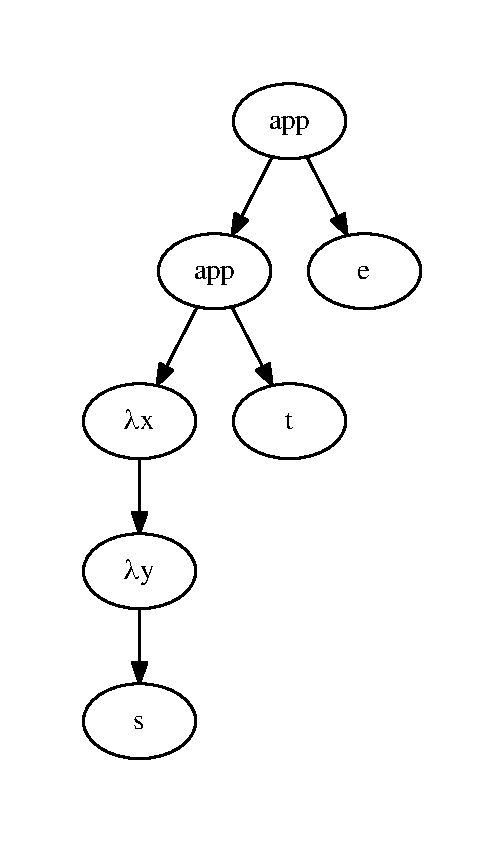
\includegraphics[width=4cm]{measure_ce1.pdf}
    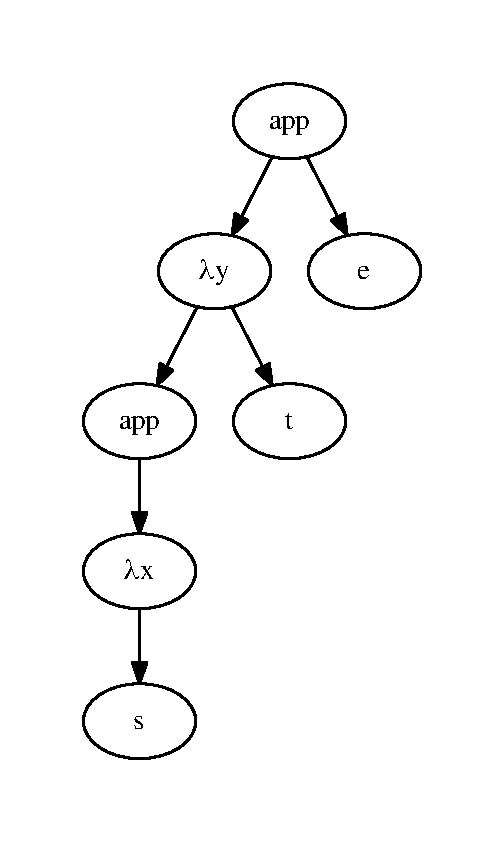
\includegraphics[width=4cm]{measure_ce2.pdf}
  \end{center}
\end{itemize}

The weight of the abstraction on $x$ decreases as expected, but at the same time
the weight of the abstraction on $y$ increases. Since $y$ is higher, its weight
contributes more.

\section{Excursion: parametrized instantiations in SANY}
\label{sec:param-inst}

In SANY, parametrized instantuitions have a representation where the
parameter is shifted over the instantiation. Let us consider the
modules Foo and Bar:

\begin{parcolumns}{2}
  \colchunk{
    \begin{lstlisting}
      ---- MODULE Foo ----

      VARIABLE a

      D(u) == u' # a'
      E(u) == D(u) \/ ENABLED D(u)

      ====
    \end{lstlisting}
  }
  \colchunk{
    \begin{lstlisting}
      ---- MODULE Bar ----
      EXTENDS Naturals

      VARIABLE x

      I(v) == INSTANCE Foo WITH a <- x+v

      ====
    \end{lstlisting}
  }
\end{parcolumns}

The term \tla{I(x)!E(x)} is represented as \tla{I!E(x,x)} but they are
not equivalent. In the meta-notation, they would be
E\{u $\mapsto$ x\}[a $\mapsto$ x+v]\{v $\mapsto$ x\} vs. E\{u $\mapsto$ x,
v $\mapsto$ x\}[a $\mapsto$ x+v] with the same consequences as in the
introduction.

\vspace{2cm}
\todo[inline]{ compute the set of unfolded defs}
\todo[inline]{ $(ENABLED\; A) \Leftrightarrow  C$ used instantiated }
\end{document}
